\documentclass[12]{article}
\usepackage[margin=1.0in]{geometry}
\usepackage[utf8]{inputenc}
\usepackage{titlesec}
\usepackage{physics}
\usepackage[version=4]{mhchem}
\usepackage{graphicx}
\usepackage{siunitx}
\usepackage{cancel}
\usepackage{amsmath}
\usepackage{textcomp}
\usepackage{gensymb}
\usepackage{natbib}
\usepackage{bm}
%\addbibresource{references.bib}

\titleformat*{\subsection}{\normalfont\fontfamily{phv}}
%\titleformat*{\subsection}[runin]{}{}{}{}[]
  \titleformat{\subsection}[runin]{\normalfont\bfseries}{\thesubsection.}{3pt}{}
  \titleformat{\subsubsection}[runin]{\normalfont\bfseries}{\thesubsubsection.}{3pt}{}

\title{{\textsc{\Large Nuclear Power Plant Shutdown Impact on Particulate Matter and Ozone across the United States}}}
\author{\textsc{Lyssa Freese}
\\\\
Advised by Prof. Noelle Selin}

\begin{document}
\maketitle
\thispagestyle{empty}

\setlength{\leftskip}{1.1cm}
\setlength{\rightskip}{1.1cm}


\bigskip
\bigskip

{\textsc{Abstract.} 
The United States’ future energy mix is likely to transition from its current 20\% reliance on nuclear power. This is due to policy changes and to scheduled shutdowns of nuclear power plants that have reached the end of their lifetime. Given projected growth in demand, the base-load nature of nuclear power, and the intermittency of most renewable resources, fossil fuel-based energy will make up at least part of this deficit, impacting air quality and the associated health impacts. We develop and validate a generator-level energy grid optimization and emissions model, and couple it with the chemical transport model, GEOS-Chem, to estimate the impact that an immediate shutdown of nuclear power plants would have on concentrations of ozone and fine particulate matter (\ce{PM_{2.5}}).

When compared to a business-as-usual scenario, the nuclear shutdown scenario leads to a nationwide 49\% increase in \ce{NO_x} emissions and a 45\% increase in \ce{SO2} emissions by coal; and a 40\% increase in \ce{NO_x} emissions by natural gas. We find \ce{PM_{2.5}} increases an average of 0.4\% nationwide, with maximum local increases of up to 33\%; summertime ozone increases an average of 0.11\%, with maximum local increases of up to 16\%. Summertime ozone decreases in small regions with volatile organic compound-limited chemical regimes, including Pittsburgh, Sacramento, Bismarck and Portland. This suggests that rapidly shutting down nuclear power plants shifts the current generation mix towards dirtier fuel sources, degrading air quality nationwide. Realistically, shutdowns will occur over longer timescales during which new generation will be deployed; this work indicates the importance of prioritizing renewable deployment as new sources of generation in order to reduce these impacts. Importantly, our generator-level energy grid optimization model allows us to assess variations across the scenarios at the local scale, which occur due to a combination of local fuel sources, demand patterns, and chemical regimes. 
 .}

\bigskip
\bigskip 
\clearpage
\setcounter{page}{1}

\setlength{\leftskip}{0cm}
\setlength{\rightskip}{0cm}

\section{Introduction}
In 2018, the United States relied on nuclear power for 19\% of electricity generation; by 2050, this is expected to decrease to only 12\% \citep{eia_annual_2020}. This is due to lower natural gas prices and declining costs of renewables, as well as increasing maintenance costs of nuclear power plants \citep{davis_market_2016}. Nuclear power has played an important role in the U.S. grid over the past few decades, providing energy that has the lowest CO2 emissions (both direct and indirect); and minimal effects on human health due to air pollution \citep{markandya_electricity_2007}. 

Previous work has shown that nuclear shutdowns tend to lead to increased use of fossil fuels, as was seen in the 2012 shutdown of San Onofre’s Nuclear Plant leading to increased use of natural gas, and Tennessee Valley’s Browns Ferry and Sequoyah 1985 shutdowns which were replaced with coal use \citep{davis_market_2016,severnini_impacts_2017}. Fossil fuels have much higher emissions of fine particulate matter (\ce{PM_{2.5}}), \ce{NO_x}, \ce{SO2}, and \ce{CO2}. \ce{NO_x} and \ce{SO2} are precursors for both ozone and \ce{PM_{2.5}}, both of which are harmful to human health. Therefore, the energy transition that will occur over the next few decades is critical to understand, and currently there is a lack of literature looking into future emission and health impacts of reducing the role of nuclear power in the U.S. energy market. 

Previous work focuses on the nation-wide health and global climate impact of U.S. energy transitions, particularly the current trend of moving from coal to natural gas \citep{lueken_climate_2016, zhang_climate_2016}, as well as the use of renewables such as wind and solar \citep{millstein_climate_2017}. These studies find \ce{SO2} and \ce{NO_x} reductions from 2016 baselines of up to 90\% and 60\%, respectively, across the United States, with a range of \$20-50 billion reductions in damages to human health \citep{lueken_climate_2016}. 

However, there are two general gaps with the current approaches to these assessments. The first is that there is little work looking at the future of nuclear power, specifically shutdowns, and what this will mean for emissions across the United States. The second is that existing work tends to focus on the national level, providing health assessments and emissions changes in national terms. Given the importance of locality to specific plants and their emissions and the fact that local state and city authorities can play an important role in energy decision-making, we find it important to think about this issue in a way that can be assessed not only nationally, but at a regional and local level as well. 


\section{Methods}

\begin{figure}[!htb]
    \centering 
    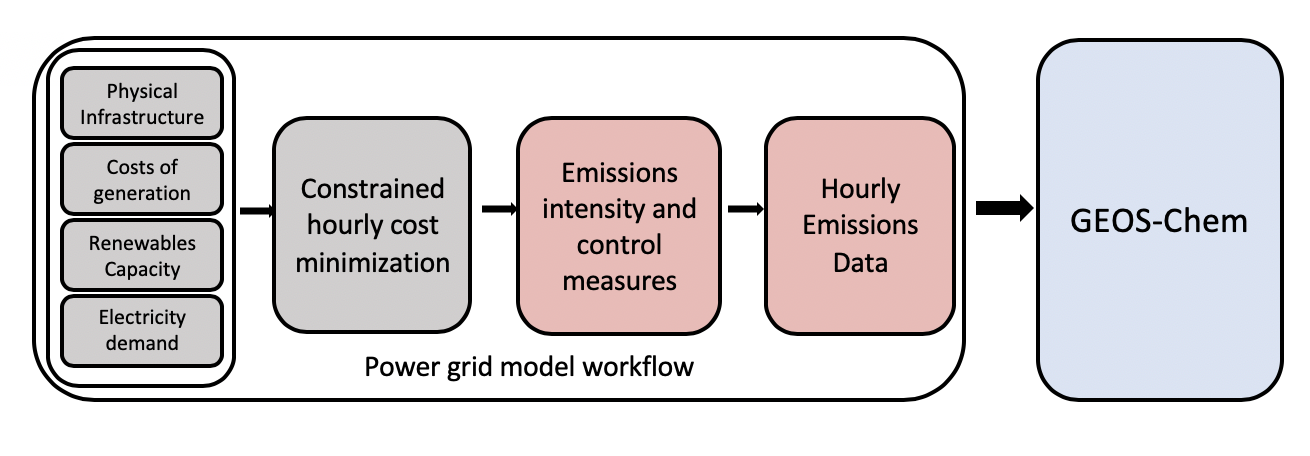
\includegraphics[scale = .5]{US_EGO_flow.png}
    \caption{US-EGO model workflow.}
    \label{fig:my_label}
\end{figure}

\subsection{US Energy Grid Optimization Model (US-EGO).}
The energy grid optimization model is a generator-level cost optimization tool, initially developed by Alan Jenn at U.C. Davis for national level assessments. A student in the Aero-Astro department took this initial framework and build a simple model for the U.S., which I assisted in developing.  

US-EGO takes all energy generating units (EGU's) across the United States, their capacity, emission factors (for \ce{CO2}, \ce{SO2}, and \ce{NOx}), and their costs for the year 2016, all of which are based on the EPA's National Electric Energy Data System (NEEDS) model v.5.16 \citep{epa_power_2016}. Separating the nation into NEEDS' 64 regions, we use 2016 transmission data (from the NEEDS data) to allow for transmission between each region, and 2016 loads to create demand within each region. The model then optimizes the use of EGUs such that the load matches generation at every hour in every region. The optimization runs across $t$ time periods with 1. $x_gen$ generation for generator $i$ at cost $c_i$ with $N$ total generators, and 2. $x_trans$ transmission power between regions d and o at cost $c_{o\rightarrow{}d}$. This is run for 8760 hours throughout the year, optimizing at each timestep \citep{jenn_future_2018}
\begin{equation}
    \min\limits_{x^{gen}, x^{trans}}\sum_{i=1}^{n}\sum_{t=1}^{T} x^{gen}_{i}(t)*c^{gen}_{i}(t) + \sum_{o,d}\sum_{t=1}^{T} x^{trans}_{o\rightarrow{}d}(t)*c^{trans}_{o\rightarrow{}d}(t)
\end{equation}

The model returns hourly output of generation, from which we calculate the hourly emissions of \ce{SO2} and \ce{NOx}. These hourly emissions are merged onto a 0.5\degree by 0.625\degree grid. 

In order to generate the no-nuclear scenario, we remove all nuclear power plants from the possible EGUs. In this scenario, generation cannot match the U.S. energy demand in the summertime in the ERC-REST region (eastern Texas), and therefore we close the gap by adding generators that have prohibitive costs such that they are only utilized when the optimization cannot close. These generators have zero emissions, and are there to allow for the optimization to close, and thus we assume partial blackouts in ERC-REST  without nuclear power during those time periods.

\subsection{Chemical Transport Model: GEOS-Chem}
We use the GEOS-Chem model \citep{} version 12.6.1 \citep{noauthor_geos-chem_2019} to simulate \ce{SO2}, \ce{NOx}, \ce{PM_{2.5}} and ozone concentrations. We use a global horizontal resolution of 4\degree x 5\degree to create boundary conditions for a nested North American run with horizontal resolution of 0.5\degree by 0.625\degree between 140\degree - 40\degree W and 10\degree - 70\degree N. We run full-chemistry in the troposphere only, with 47 vertical levels. Our spin-up is four months, and we analyze daily concentration outputs for the year of 2016. 

We run four GEOS-Chem simulations with different U.S. EGU emission inputs: default, e-grid, US-EGO, and no-nuclear. The default simulation takes the standard GEOS-Chem U.S. EGU emissions files, which are taken from the National Emissions Inventory (NEI) 2011 emissions scaled to the year 2013. The e-grid simulation utilizes the EPA's Emission and Generation Resource Integrated Database (e-grid) \citep{epa_emissions_2016} \ce{SO2} and \ce{NOx} emissions gridded onto a 0.5\degree by 0.625\degree grid. The US-EGO simulation uses the emissions profiles created through the US-EGO model, and the no-nuclear scenario uses emissions profiles created through the US-EGO model in a no nuclear scenario. 


\section{Results and Discussion}
\subsection{Model Validation}

In order to validate the model, we compare our emissions output to that of the EPA's e-grid, and the NEI 2011 data, scaled to the 2013 values as is done in GEOS-Chem. We compare the emissions profiles before running it through GEOS-Chem, and the resulting concentrations as obtained from these three GEOS-Chem scenarios. Additionally, we compare the annual mean GEOS-Chem concentrations of each model run to the EPA Air Quality System (AQS) monitoring data for 2016. 

Our model emissions by region and fuel-type correlates reasonably well with the emissions by region and fuel-type from both the e-grid and NEI (Figure***), which indicates that the optimization does an adequate job of capturing the emissions of energy generating units across the United States in the year 2016. We find bias in x regions during x times ***.

From this, we can have confidence that our model 
\subsection{Ozone impacts of a no-nuclear scenario}

Figure *** shows the seasonal changes in \ce{SO2} and \ce{NOx} concentrations across the United States, and regionally. We define the summer season as June, July and August (JJA), and winter as December, January, and February (DJF) We see increases in \ce{NOx} emissions nationwide throughout the entire year, with 


\subsection{\ce{PM_{2.5}} Trends}

\section{Future work}



\section{Acknowledgements}


\pagebreak
\bibliographystyle{apalike}
\bibliography{references.bib}

\end{document}

